\documentclass[12pt]{article}

\usepackage[english]{babel}
\usepackage{geometry}
\usepackage{fontspec}
\usepackage{import}
\usepackage{graphicx}
\usepackage{titlesec}
\usepackage{caption}
\usepackage{subcaption}
\usepackage{float}
\usepackage{fancyhdr}
\usepackage{xcolor}
\usepackage{enumitem}
\usepackage{mathtools}
\usepackage{amsmath}
\usepackage{unicode-math}
\usepackage{amsthm}
\usepackage{physics}
\usepackage{xfrac}
\usepackage{multirow}
\usepackage{colortbl}
\usepackage{longtable}
\usepackage{booktabs}
\usepackage{etoolbox}
\usepackage{minted}
\usepackage{listings}
\lstset{
    language=Python,
    basicstyle=\ttfamily\small,
    keywordstyle=\color{blue},
    commentstyle=\color{gray},
    stringstyle=\color{red},
    numbers=left,
    numberstyle=\tiny\color{gray},
    frame=single,
    breaklines=true,
    xleftmargin=2em,
    framexleftmargin=1.5em
}
\usepackage{csquotes}
\usepackage[nottoc]{tocbibind}
\usepackage{tocloft}
\usepackage{ktu}
\usepackage{hyperref}

\begin{document}

\begin{titlepage}
    \newcommand{\module}{P176B106 Machine Learning Algorithms 2}
    \newcommand{\worktitle}{Smart Traffic Light Control using Reinforcement Learning}
    \newcommand{\type}{Report of Engineering Project}
    \newcommand{\professor}{Dalia Čalnerytė}
    \newcommand{\university}{Kaunas University of Technology}
    \newcommand{\faculty}{Faculty of Informatics}
    \newcommand{\professortitle}{Lecturer}
    \newcommand{\city}{Kaunas}
    \newcommand{\workyear}{\the\year}

    \centering
    
\includegraphics[width=0.12\textwidth]{images/ktu-logo.pdf} \\ ~ \\

    \textbf{\university} \\
    {\faculty} \\

    \vfill

    {\Large \textbf{\worktitle}} \\
    ~\\
    {\large \type}
    ~\\~\\
    {\large \module}

    \vfill

    \flushright
    {
        \begin{tabular}{l}
            \textbf{Leonid Oliinyk} \\
            \textbf{Mykhailo Soroka} \\
            \textbf{Dániel Apró} \\
            Students \\
            ~ \\
            \textbf{\professor} \\
            \professortitle
        \end{tabular}
    }

    \vfill

    \centering
    \textbf{\city, \workyear}
\end{titlepage}

\setcounter{page}{2}


\tableofcontents

\phantomsection
\section*{Introduction}
\addcontentsline{toc}{section}{Introduction}

Urban traffic congestion imposes significant economic and environmental costs: vehicles
idling at intersections waste fuel, increase emissions, and reduce overall road throughput.
Traditional fixed-time traffic signal controllers allocate green time according to
pre-programmed schedules that cannot adapt to real-time demand fluctuations, particularly
during off-peak hours or unexpected events.

Reinforcement Learning (RL) offers a principled framework for adaptive signal control.
An RL agent interacts with a traffic environment, observing the current state of queues
and flows, choosing a signal phase, and receiving a reward that encodes how good the
outcome was. Over many episodes the agent learns a policy that minimises vehicle waiting
times without requiring a hand-crafted schedule.

This work implements \textbf{Tabular Q-Learning} for a single signalised intersection
simulated in the SUMO microscopic traffic simulator via the \texttt{sumo-rl} Gymnasium
wrapper. Two reward configurations are compared: the default differential waiting-time
reward and a custom quadratic queue-length penalty. The report describes the system
architecture, the RL method, the experimental setup, and a quantitative comparison of
both configurations across 50 training episodes.

\newpage

\section{System Architecture}

The system consists of four loosely coupled components as illustrated conceptually below.

\textbf{SUMO Simulator.} Eclipse SUMO (Simulation of Urban MObility, version 1.18.0)
provides a microscopic simulation of individual vehicle movements, traffic-signal
phases, and inter-vehicle interactions. It is controlled via the TraCI protocol,
which exposes a Python API for retrieving sensor data and issuing phase commands.

\textbf{sumo-rl Environment.} The \texttt{sumo-rl} library (version 1.4.5) wraps SUMO
as a standard Gymnasium environment. It handles episode resets, TraCI communication,
observation assembly, and optional CSV logging of per-step metrics. The agent interacts
with it through the standard \texttt{reset()} / \texttt{step()} interface using the
five-tuple unpacking introduced in Gymnasium 0.26:
\begin{lstlisting}
next_obs, reward, terminated, truncated, info = env.step(action)
\end{lstlisting}

\textbf{Q-Learning Agent.} A dictionary-based Q-table maps discrete state tuples to
arrays of action values. The agent encapsulates state discretisation, action selection
(epsilon-greedy), and the Bellman update. No external ML library is required.

\textbf{Analysis Pipeline.} After training, the per-step CSV files written by
\texttt{sumo-rl} are parsed with \texttt{pandas} to compute per-episode summaries.
\texttt{matplotlib} generates all plots.

\newpage

\section{Environment Description}

\subsection{Network and Route Files}

The simulation uses the \texttt{single-intersection} network bundled with \texttt{sumo-rl}.
It models a four-way intersection with one lane per approach (North, South, East, West).
Vehicles are spawned stochastically according to a pre-defined route file that maintains
a steady mixed-direction demand throughout the 3\,600-second episode duration.

\subsection{Observation Space}

At each decision step the environment returns an 11-dimensional continuous observation
vector. The first eight elements are the normalised lane density and queue length for each
of the four incoming lanes — values in $[0,1]$ representing the fraction of lane capacity
occupied and the fraction of vehicles that are stationary, respectively. The remaining
three elements encode phase timing information. The full vector is:
\begin{equation}
    \mathbf{o} = \bigl[
        \rho_N,\, \rho_S,\, \rho_E,\, \rho_W,\;
        q_N,\, q_S,\, q_E,\, q_W,\;
        \phi_1,\, \phi_2,\, \phi_3
    \bigr] \in [0,1]^{11}
\end{equation}
where $\rho_i$ is lane density, $q_i$ is normalised queue length, and $\phi_j$ encodes
current phase/timing state.

\subsection{Action Space}

The agent selects one of two green phases at each decision step:
\begin{itemize}[noitemsep]
    \item \textbf{Action 0} — North--South green, East--West red.
    \item \textbf{Action 1} — East--West green, North--South red.
\end{itemize}
The environment enforces a minimum green time of 5\,s and inserts a 2\,s yellow
transition automatically between any phase change.

\subsection{Reward Functions}

Two reward configurations are evaluated:

\textbf{Configuration A — Default reward} (differential waiting time):
\begin{equation}
    r_t = \sum_{i} W_i^{t-1} - \sum_{i} W_i^{t}
\end{equation}
where $W_i^t$ is the accumulated waiting time of vehicle $i$ at step $t$.
A positive reward means total waiting decreased this step.

\textbf{Configuration B — Quadratic queue penalty}:
\begin{equation}
    r_t = -\!\left(\sum_{l} h_l^t\right)^{\!2}
\end{equation}
where $h_l^t$ is the number of halting vehicles in lane $l$ at step $t$.
Squaring amplifies the cost of large backlogs non-linearly, incentivising the
agent to clear congested lanes quickly even at the expense of lighter queues.

\subsection{Episode Structure}

Each episode simulates 3\,600 seconds of traffic. With \texttt{delta\_time}~$=5$\,s,
the agent makes 720 decisions per episode. The simulation clock restarts at \texttt{reset()}.

\newpage

\section{Tabular Q-Learning}

\subsection{State Discretisation}

The continuous observation vector cannot be used directly as a Q-table key.
Each of the 11 features is mapped to one of $B = 4$ bins by dividing $[0,1]$
into equal-width intervals with boundaries $\{0.25,\, 0.50,\, 0.75\}$:
\begin{equation}
    d_j = \mathrm{clip}\!\left(\lceil 4 x_j \rceil - 1,\; 0,\; 3\right)
          \quad \text{for each feature } x_j \in [0,1]
\end{equation}
The resulting 11-dimensional integer tuple $(d_0,\dots,d_{10})$ is used as a
Python dictionary key. The theoretical state-space size is $4^{11} = 4{,}194{,}304$,
but in practice only a small fraction of states is visited; after 50 training episodes,
the Q-table contained 293 states for Configuration A and 321 for Configuration B.

\subsection{Q-Learning Update}

The agent applies the standard Bellman equation at every decision step:
\begin{equation}
    Q(s,a) \;\leftarrow\; Q(s,a) \;+\; \alpha \Bigl[
        r \;+\; \gamma \max_{a'} Q(s',a') \;-\; Q(s,a)
    \Bigr]
    \label{eq:bellman}
\end{equation}
where $\alpha$ is the learning rate, $\gamma$ the discount factor, $r$ the immediate
reward, $s'$ the next state, and $a'$ ranges over all actions. New states are
initialised with $Q = 0$ (optimistic initialisation would require prior knowledge
of reward magnitudes).

\subsection{Exploration Strategy}

Action selection uses an $\varepsilon$-greedy policy. At episode $e$:
\begin{equation}
    \pi(s) = \begin{cases}
        \text{random action} & \text{with probability } \varepsilon_e \\
        \arg\max_{a} Q(s,a) & \text{otherwise}
    \end{cases}
\end{equation}
with $\varepsilon_e = \max(\varepsilon_{\min},\; \varepsilon_0 \cdot \delta^{e-1})$.
Ties in $\arg\max$ are broken by adding negligible Gaussian noise, ensuring uniform
tie-breaking without a separate random-action call.

\subsection{Hyperparameters}

\begin{table}[H]
    \centering
    \caption{Q-Learning hyperparameters used in all experiments}
    \label{tab:hyperparams}
    \begin{tabular}{lll}
        \toprule
        \textbf{Parameter} & \textbf{Symbol} & \textbf{Value} \\
        \midrule
        Learning rate          & $\alpha$             & 0.10 \\
        Discount factor        & $\gamma$             & 0.95 \\
        Initial exploration    & $\varepsilon_0$      & 1.00 \\
        Exploration decay      & $\delta$             & 0.98 \\
        Minimum exploration    & $\varepsilon_{\min}$ & 0.05 \\
        Observation bins       & $B$                  & 4    \\
        Training episodes      & —                    & 50   \\
        Episode duration       & —                    & 3\,600\,s \\
        Decision interval      & \texttt{delta\_time} & 5\,s \\
        Yellow phase           & \texttt{yellow\_time}& 2\,s \\
        Minimum green          & \texttt{min\_green}  & 5\,s \\
        \bottomrule
    \end{tabular}
\end{table}

\newpage

\section{Evaluation Strategy}

\subsection{Metrics}

Three metrics are tracked from the \texttt{sumo-rl} per-step CSV logs after each episode:
\begin{itemize}[noitemsep]
    \item \textbf{Average queue length} — mean number of halting vehicles per step.
    \item \textbf{Maximum queue length} — peak number of halting vehicles in the episode.
    \item \textbf{Average waiting time} — mean per-vehicle waiting time across all steps (seconds).
\end{itemize}
Lower values indicate better performance for all three metrics.

\subsection{Visualisations}

Four types of plot are produced for each configuration:

\begin{enumerate}[noitemsep]
    \item \textbf{Training reward curve} — per-episode total reward with a rolling-mean
          smoothing window of $\lfloor 0.2 \times 50 \rfloor = 10$ episodes.
    \item \textbf{Performance metrics} — average queue (with max band) and average waiting
          time per episode, enabling direct comparison between configurations.
    \item \textbf{Signal-schedule visualisation} — a three-panel figure for episode 1
          (random policy) and the final episode (trained policy), showing:
          (a) a Gantt chart of active phases, (b) total stopped vehicles over time,
          and (c) a heatmap of the full observation vector — the agent's ``view'' of
          traffic state at every decision step.
    \item \textbf{Q-table heatmap} — all visited states projected onto the first two
          observation dimensions, coloured by estimated state value and preferred action.
\end{enumerate}

\newpage

\section{Experiments and Results}

\subsection{Training Reward Curves}

Figure~\ref{fig:reward} shows the per-episode total reward for both configurations
across 50 training episodes. Both curves begin at their most negative values,
reflecting the random exploration of the first episodes ($\varepsilon_1 = 1.0$), and
trend upward as the Q-table accumulates experience.

The quadratic configuration (orange) converges faster in early episodes, likely because
its larger penalty magnitude ($-q^2$ vs.\ differential reward) creates steeper gradients
that reinforce clearly good decisions more strongly. By episode 30, both curves approach
a similar plateau, suggesting that 50 episodes are sufficient to reach a stable policy
with the chosen hyperparameters.

\begin{figure}[H]
    \centering
    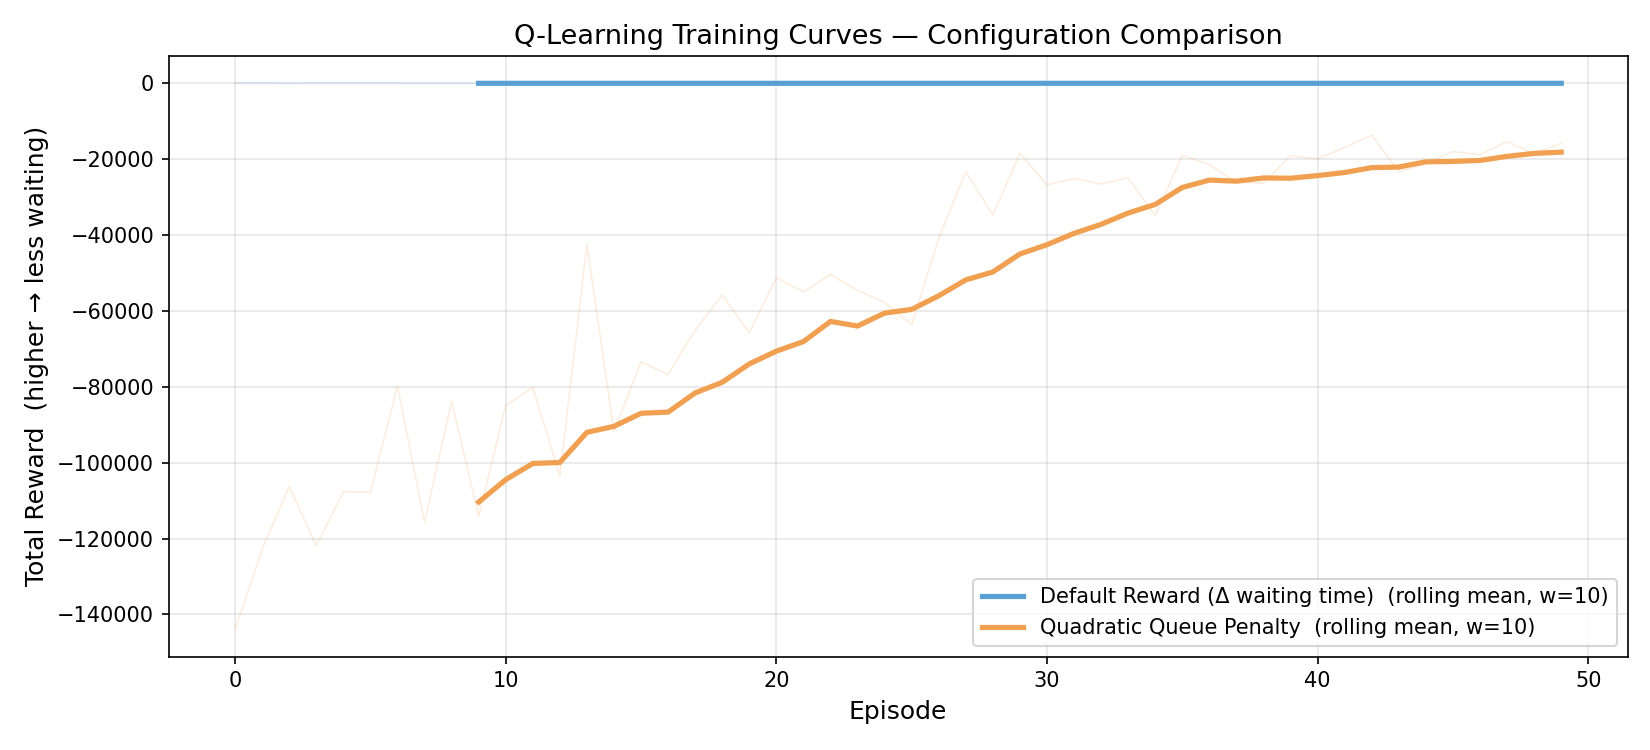
\includegraphics[width=\textwidth]{reward_comparison.png}
    \caption{Per-episode total reward for both reward configurations.
             Solid lines show 10-episode rolling means; shaded traces are raw values.}
    \label{fig:reward}
\end{figure}

\subsection{Queue Length and Waiting Time}

Figure~\ref{fig:metrics} plots the per-episode average queue length (with shaded
average-to-maximum band) and average waiting time. Both configurations show clear
monotonic improvement over training.

\begin{figure}[H]
    \centering
    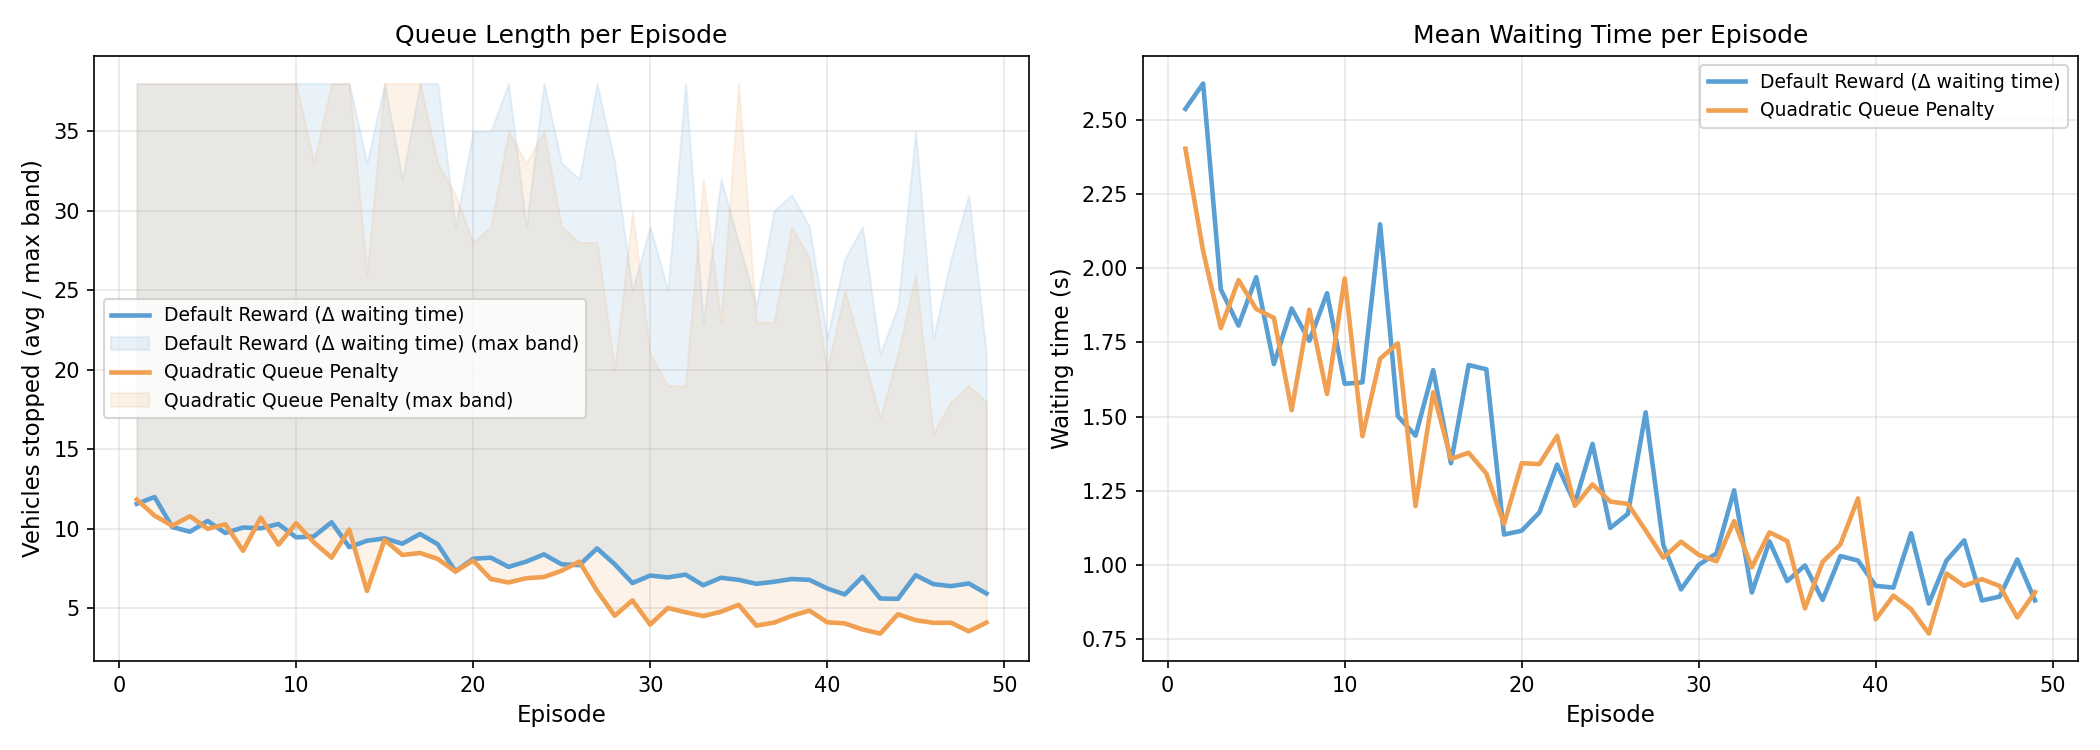
\includegraphics[width=\textwidth]{performance_metrics.png}
    \caption{Per-episode queue length (left, shaded band = avg to max) and
             mean waiting time (right) for both configurations.}
    \label{fig:metrics}
\end{figure}

Table~\ref{tab:results} summarises the quantitative improvement from episode 1
to episode 50.

\begin{table}[H]
    \centering
    \caption{Performance metrics — episode 1 vs.\ episode 50}
    \label{tab:results}
    \begin{tabular}{lrrrrrr}
        \toprule
        & \multicolumn{3}{c}{\textbf{Episode 1}} & \multicolumn{3}{c}{\textbf{Episode 50}} \\
        \cmidrule(lr){2-4} \cmidrule(lr){5-7}
        \textbf{Config} & Avg Q & Max Q & Avg Wait & Avg Q & Max Q & Avg Wait \\
        \midrule
        A — Default   & 11.57 & 38 & 2.54\,s & 5.93 & 21 & 0.88\,s \\
        B — Quadratic & 11.84 & 38 & 2.40\,s & 4.11 & 18 & 0.91\,s \\
        \bottomrule
    \end{tabular}
\end{table}

Configuration A (default) reduces average queue by \textbf{48.7\,\%} and average
waiting time by \textbf{65.3\,\%} over the course of training.
Configuration B (quadratic) achieves a larger queue reduction of \textbf{65.3\,\%},
while waiting time falls by \textbf{62.2\,\%} — a slightly lower figure, consistent
with the quadratic penalty optimising queue counts rather than individual waiting times directly.

\subsection{Signal Schedule — Beginning vs.\ End of Training}

Figures~\ref{fig:sched_default} and~\ref{fig:sched_quadratic} show the signal schedule
visualisation for both configurations at episode 1 (random policy) and episode 50
(trained policy).

\begin{figure}[H]
    \centering
    \begin{subfigure}[b]{0.49\textwidth}
        \centering
        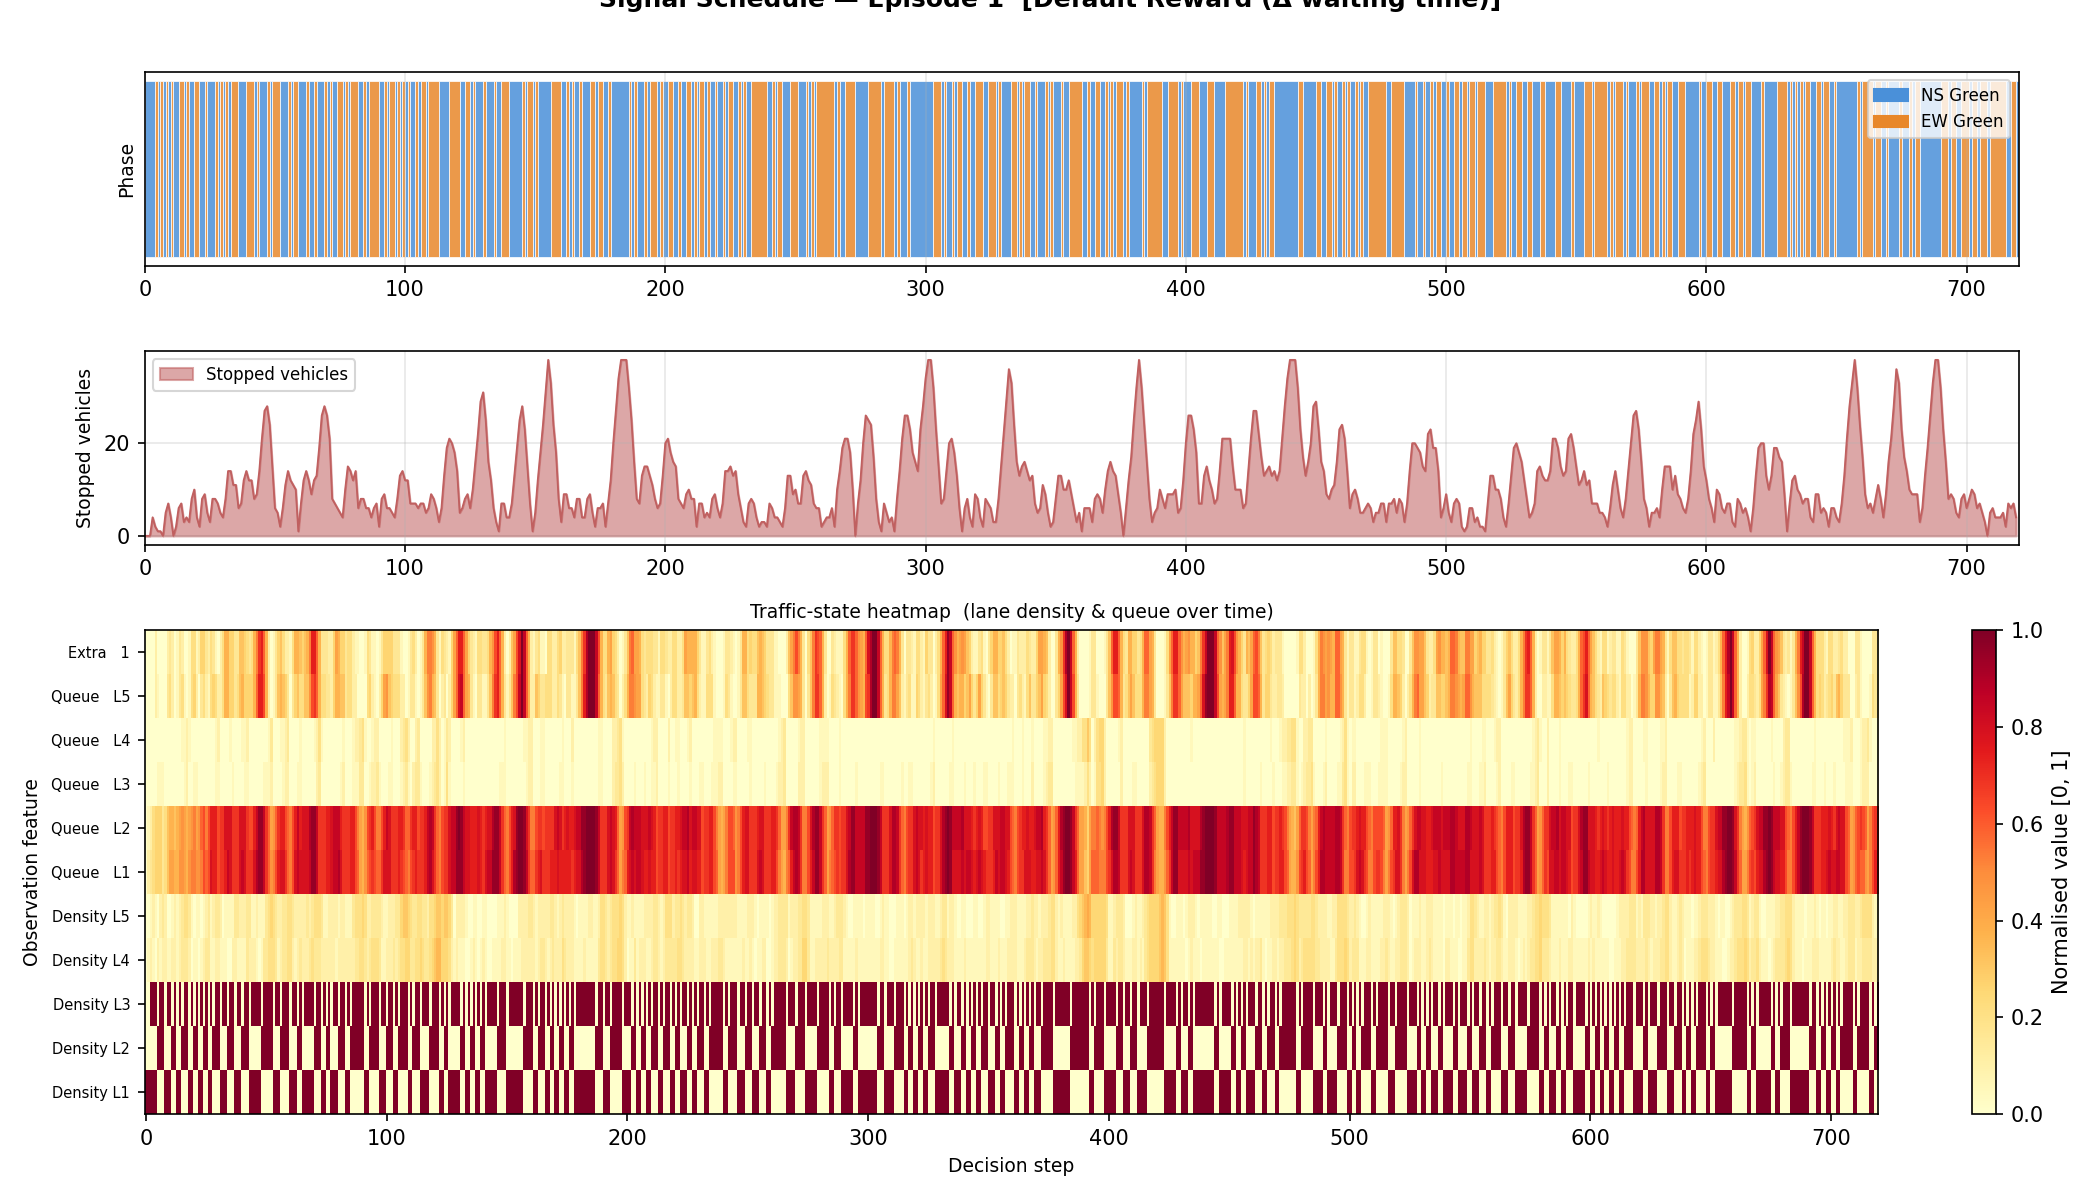
\includegraphics[width=\textwidth]{signal_schedule_default_ep1.png}
        \caption{Episode 1 (random policy)}
    \end{subfigure}
    \hfill
    \begin{subfigure}[b]{0.49\textwidth}
        \centering
        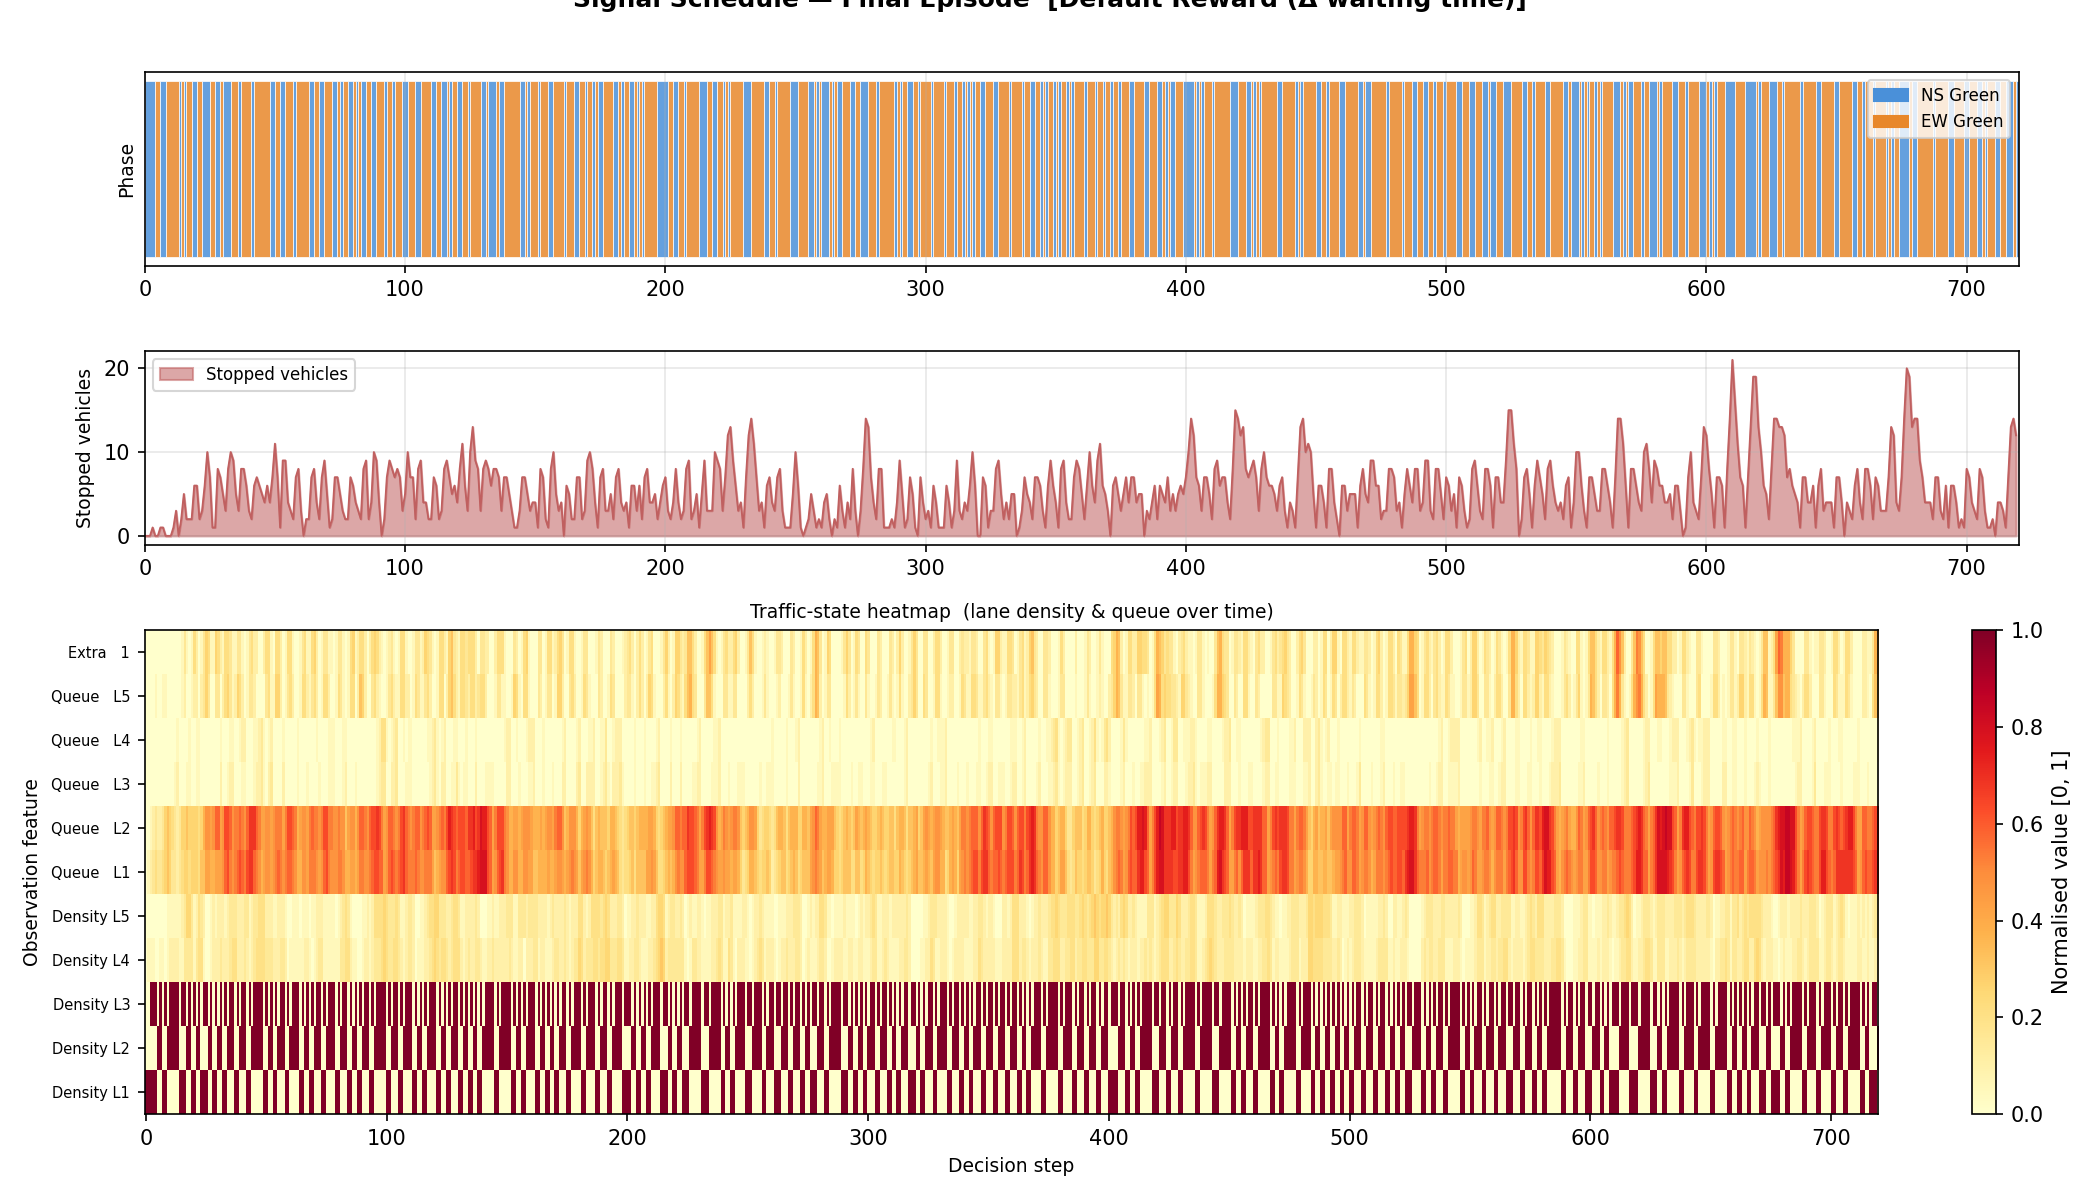
\includegraphics[width=\textwidth]{signal_schedule_default_final.png}
        \caption{Episode 50 (trained policy)}
    \end{subfigure}
    \caption{Signal schedule for Configuration A (default reward).
             Top: phase Gantt (blue = NS green, orange = EW green).
             Middle: total stopped vehicles. Bottom: observation heatmap.}
    \label{fig:sched_default}
\end{figure}

In episode 1 (random policy), the Gantt chart shows frequent, irregular phase switches
with no clear pattern, and the stopped-vehicle count grows steadily throughout the
episode, peaking near 38 vehicles. The observation heatmap shows high queue values
(red) sustained for long periods on multiple lanes simultaneously.

By episode 50 the trained agent maintains each phase for longer and more consistent
intervals, reducing unnecessary transitions. The stopped-vehicle count is lower on
average and recovers more quickly after each peak. The heatmap shows shorter high-queue
periods and a clearer alternating structure corresponding to the two phases.

\begin{figure}[H]
    \centering
    \begin{subfigure}[b]{0.49\textwidth}
        \centering
        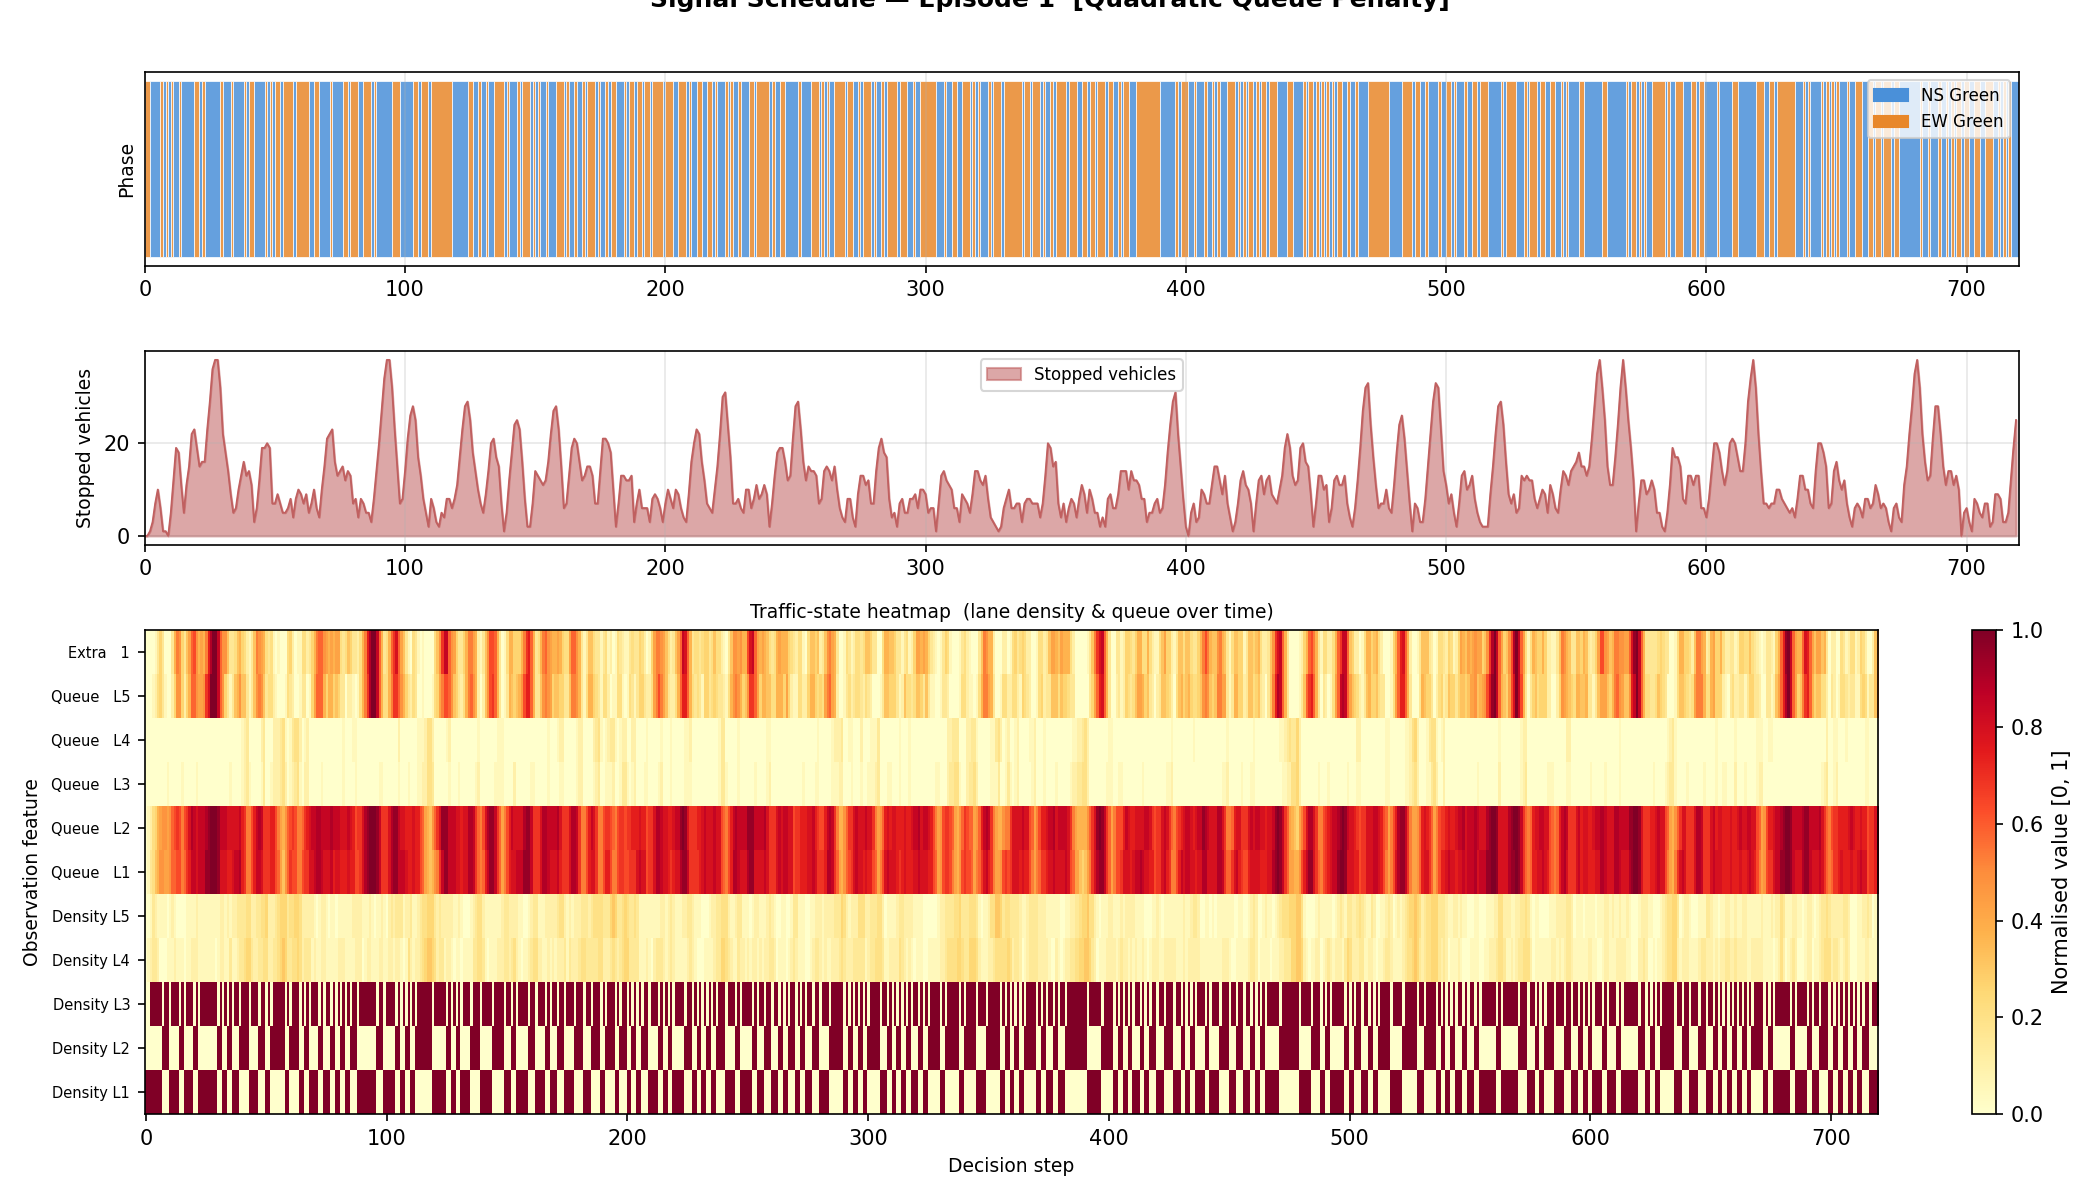
\includegraphics[width=\textwidth]{signal_schedule_quadratic_ep1.png}
        \caption{Episode 1 (random policy)}
    \end{subfigure}
    \hfill
    \begin{subfigure}[b]{0.49\textwidth}
        \centering
        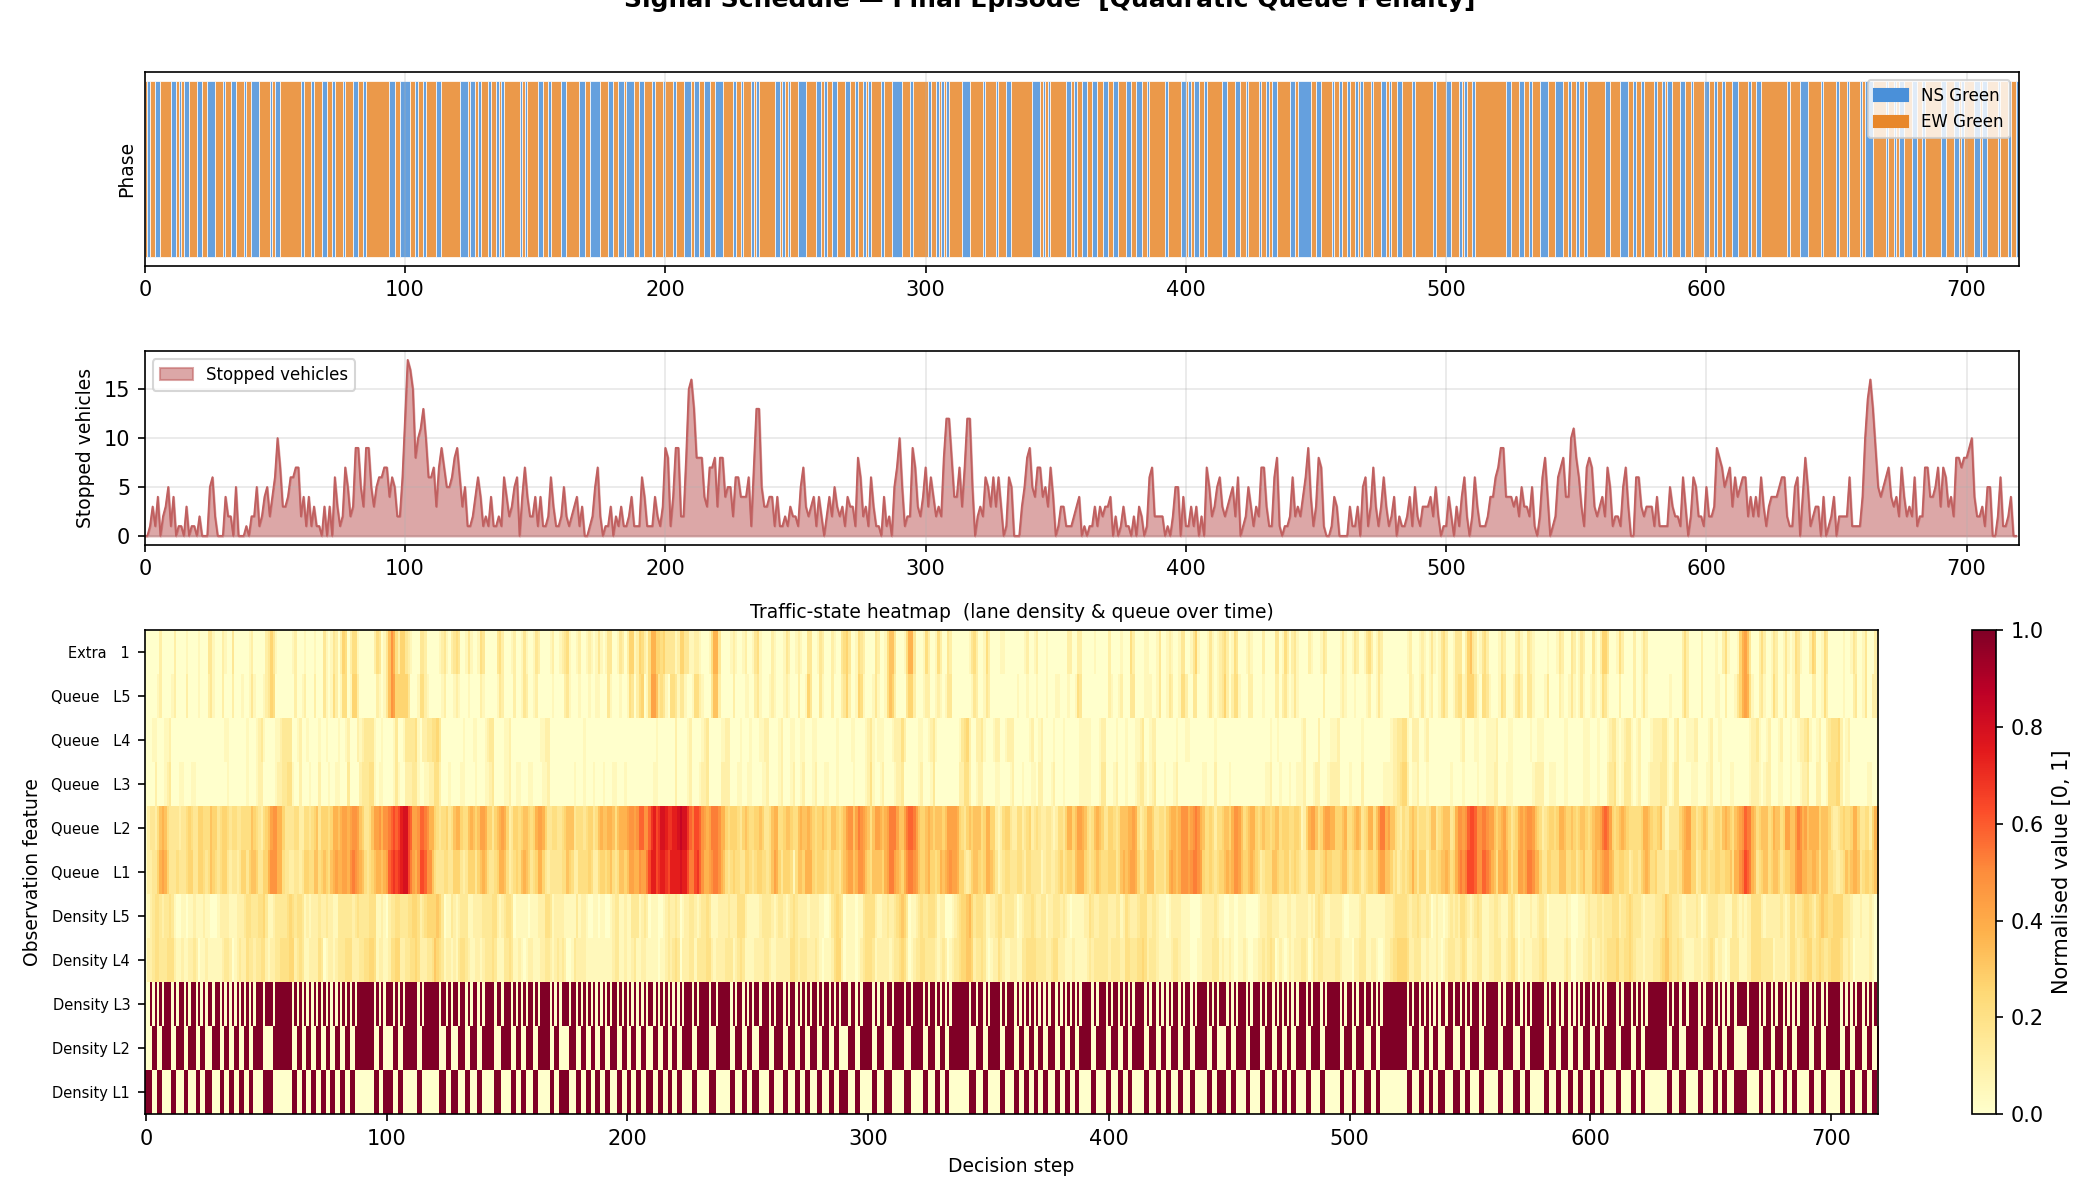
\includegraphics[width=\textwidth]{signal_schedule_quadratic_final.png}
        \caption{Episode 50 (trained policy)}
    \end{subfigure}
    \caption{Signal schedule for Configuration B (quadratic queue penalty).
             Same panel layout as Fig.~\ref{fig:sched_default}.}
    \label{fig:sched_quadratic}
\end{figure}

Configuration B shows a similar pattern: early random switching gives way to a more
deliberate policy. The quadratic reward places disproportionate cost on large queues,
so the trained agent is observed to switch to NS green more aggressively when the
EW queue grows large, visible in the observation heatmap as quicker decay of high-density
periods on the EW lanes.

\subsection{Q-Table Analysis}

Figure~\ref{fig:qtable} projects the visited Q-table states onto the first two
observation dimensions — the density bins of the North and South lanes — and colours
each state by its estimated value (left) and preferred action (right).

\begin{figure}[H]
    \centering
    \begin{subfigure}[b]{0.49\textwidth}
        \centering
        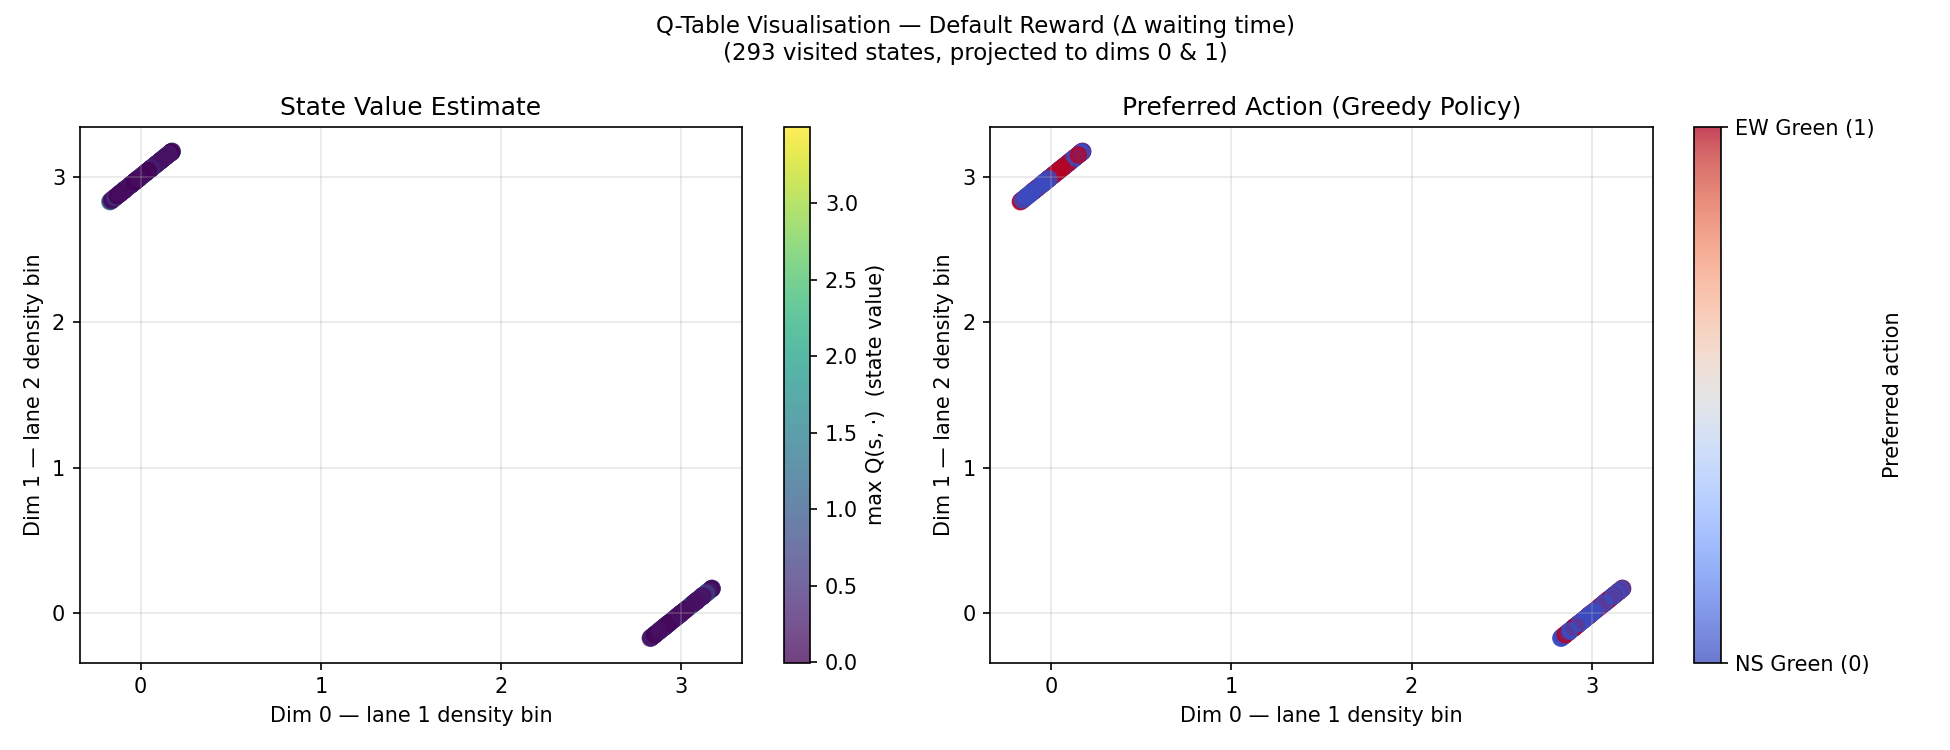
\includegraphics[width=\textwidth]{q_table_heatmap_default.png}
        \caption{Configuration A — default reward}
    \end{subfigure}
    \hfill
    \begin{subfigure}[b]{0.49\textwidth}
        \centering
        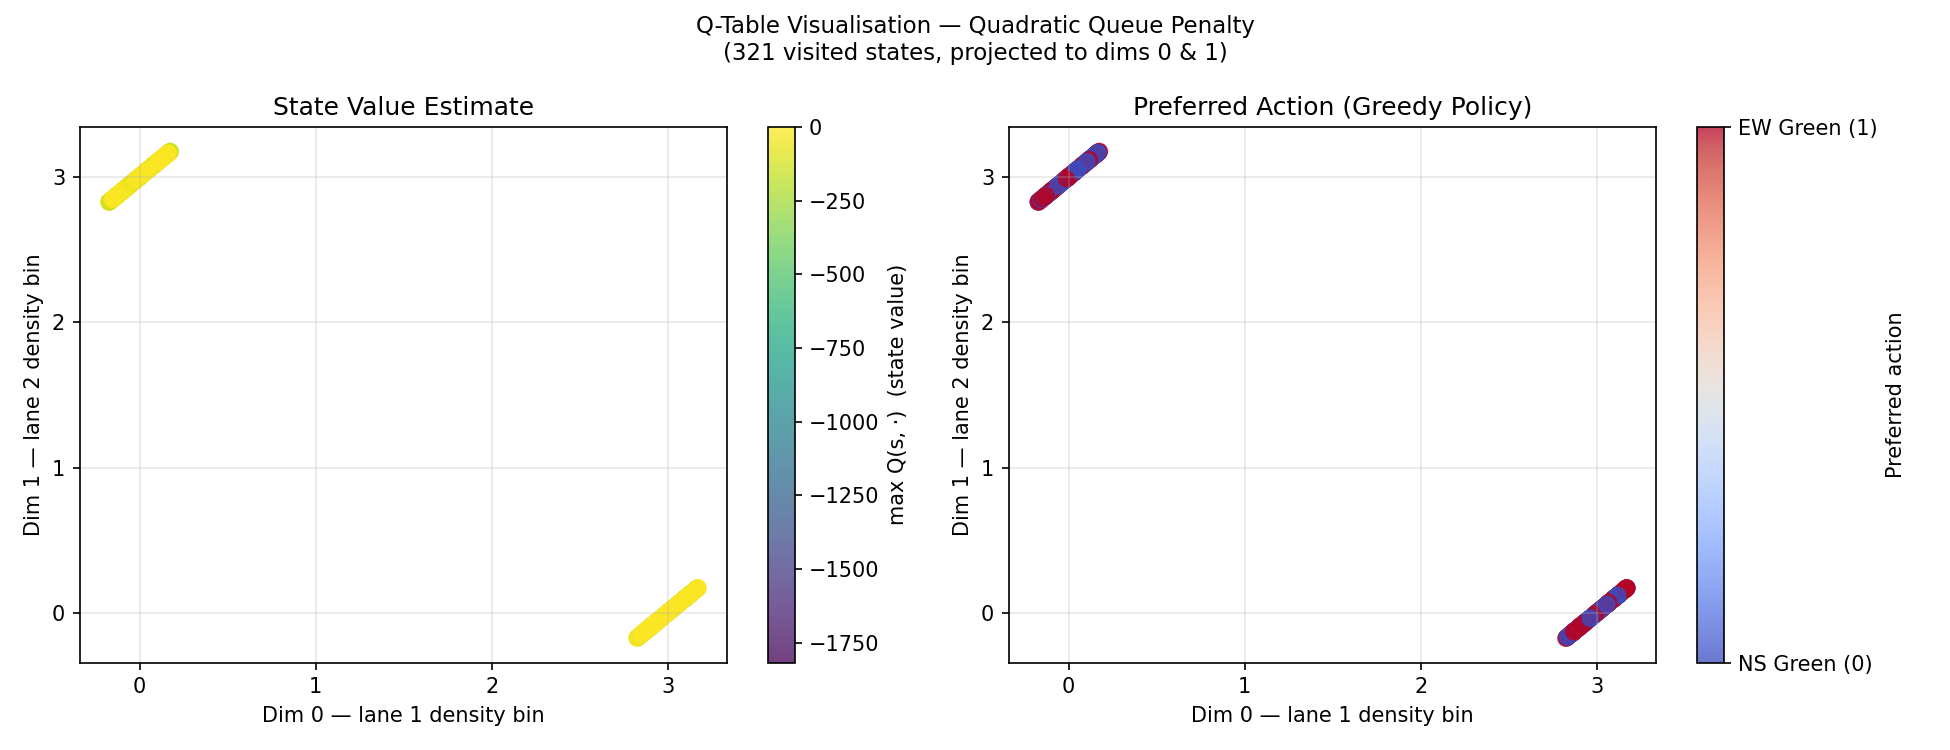
\includegraphics[width=\textwidth]{q_table_heatmap_quadratic.png}
        \caption{Configuration B — quadratic penalty}
    \end{subfigure}
    \caption{Q-table heatmaps. Left panel: estimated state value (max Q-value).
             Right panel: greedy action (0 = NS green, 1 = EW green).}
    \label{fig:qtable}
\end{figure}

Both configurations learn a similar structure: states with higher density bins in the
projected dimensions (upper-right region) tend to have lower estimated values,
corresponding to congested situations where the agent has limited ability to reduce
waiting. The preferred-action map shows that the agent learns to prefer NS green (action 0)
in low-density states and EW green (action 1) when EW demand is higher — a sensible
policy given symmetric traffic in the route file.

The quadratic configuration visited 321 unique states versus 293 for the default
configuration, suggesting broader state exploration driven by the stronger penalty
signal encouraging more active phase switching during early training.

\subsection{Final-Episode Comparison}

Figure~\ref{fig:comparison} provides a direct bar-chart comparison of the three
metrics at episode 50.

\begin{figure}[H]
    \centering
    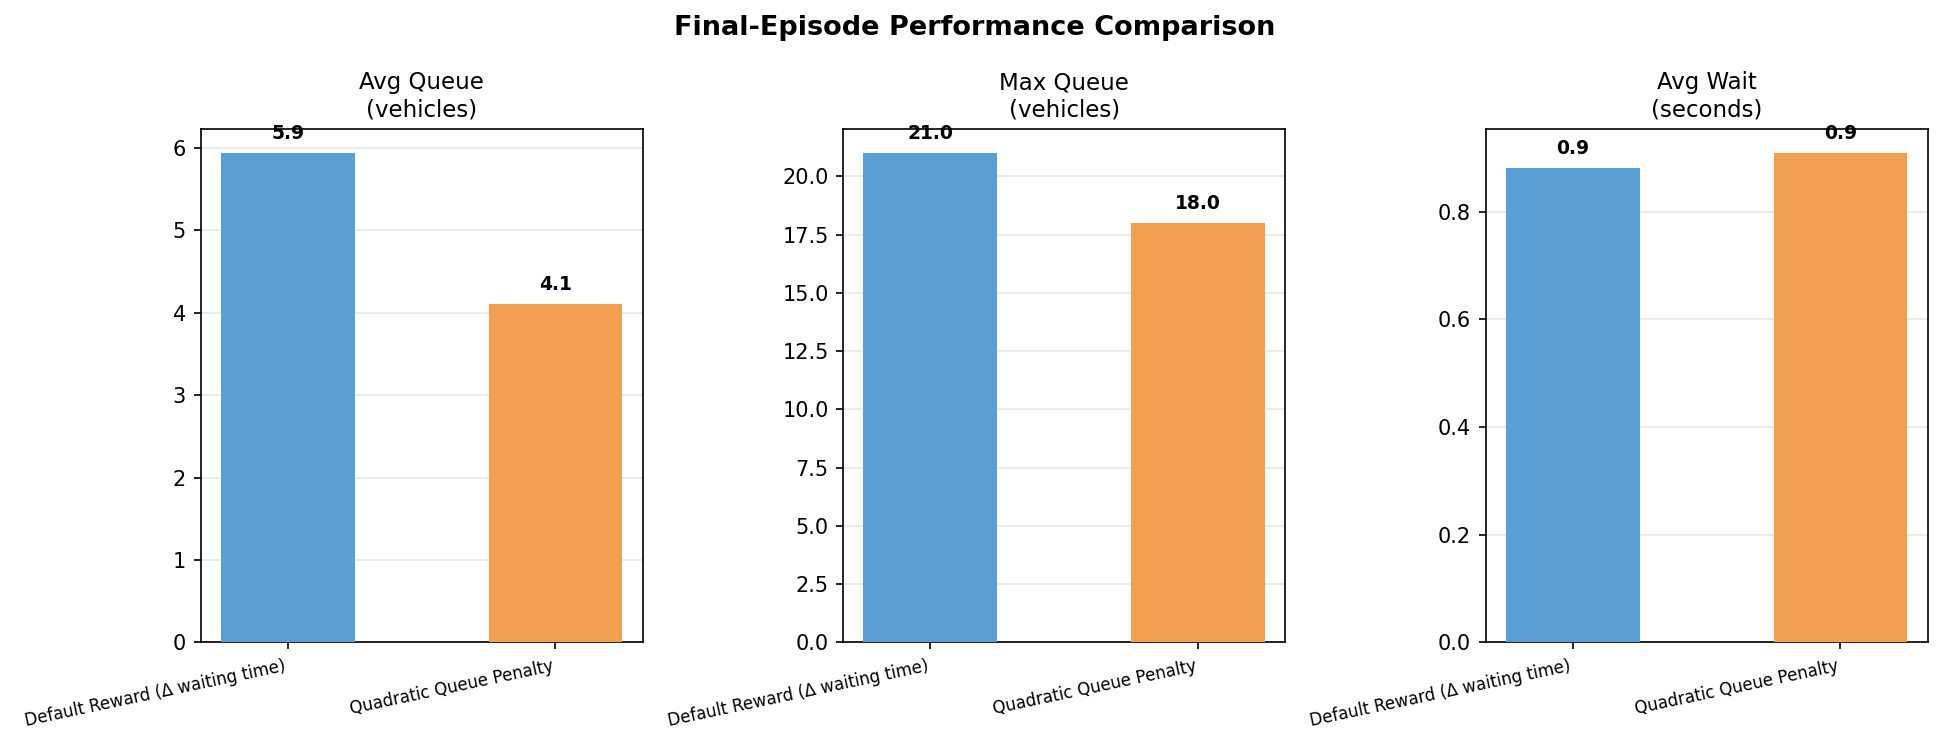
\includegraphics[width=\textwidth]{final_comparison.png}
    \caption{Final-episode performance comparison between the two reward configurations.}
    \label{fig:comparison}
\end{figure}

Configuration B (quadratic) achieves a lower average queue (4.11 vs.\ 5.93 vehicles)
and lower maximum queue (18 vs.\ 21 vehicles) than Configuration A.
Average waiting time is comparable (0.91\,s vs.\ 0.88\,s), with Configuration A
slightly better by 0.03\,s. This indicates that the quadratic penalty is more effective
at keeping queues short overall, while the differential reward is marginally better at
minimising individual vehicle delays.

\newpage

\phantomsection
\section*{Conclusions}
\addcontentsline{toc}{section}{Conclusions}

Tabular Q-Learning was applied to adaptive traffic-light control at a single SUMO
intersection, comparing two reward functions over 50 training episodes of 3\,600
simulated seconds each.

Both configurations demonstrated substantial improvement over the random policy used
in episode 1. The default differential waiting-time reward (Configuration A) reduced
average queue by 48.7\,\% and average waiting time by 65.3\,\%. The quadratic
queue-length penalty (Configuration B) achieved a larger queue reduction of 65.3\,\%
with a comparable waiting-time reduction of 62.2\,\%, and reached a lower final
average queue (4.11 vs.\ 5.93 vehicles) and maximum queue (18 vs.\ 21 vehicles).

Signal-schedule visualisations confirmed qualitative improvement: the trained policy
produces longer, more consistent phase intervals with fewer redundant transitions,
and the traffic-state heatmaps show quicker queue recovery after each phase change.
Q-table analysis revealed that both agents learn directionally sensible policies,
preferring the phase that serves the higher-demand direction, while the quadratic
agent explores a broader region of the state space.

The main limitation of Tabular Q-Learning in this setting is the dependency on
state discretisation: with 4 bins per feature and an 11-dimensional observation,
only a tiny fraction ($< 0.01\,\%$) of the theoretical state space is visited,
leaving many states with uninformed $Q = 0$ values. Function approximation methods
such as Deep Q-Networks (DQN) would generalise across unvisited states and scale
to larger networks. Future work should also include a fixed-time baseline controller
for comparison, extend the scenario to multi-intersection networks using the
multi-agent interface of \texttt{sumo-rl}, and increase the number of training
episodes to assess whether performance continues to improve beyond episode 50.

\end{document}
